\documentclass[titlepage,a4paper]{article}

\usepackage{a4wide}
\usepackage[colorlinks=true,linkcolor=black,urlcolor=blue,bookmarksopen=true]{hyperref}
\usepackage{bookmark}
\usepackage{fancyhdr}
\usepackage[spanish]{babel}
\usepackage[utf8]{inputenc}
\usepackage[T1]{fontenc}
\usepackage{graphicx}
\usepackage{float}
\usepackage{amsmath}
\usepackage{booktabs}

\pagestyle{fancy} % Encabezado y pie de página
\fancyhf{}
\fancyhead[L]{TP1 - Violeta Perez Andrade}
\fancyhead[R]{Sistemas Digitales - FIUBA}
\renewcommand{\headrulewidth}{0.4pt}
\fancyfoot[C]{\thepage}
\renewcommand{\footrulewidth}{0.4pt}
\usepackage{listings}
\usepackage{xcolor}

\lstdefinelanguage{VHDL}{
    morekeywords=[1]{
        library,use,all,entity,is,port,in,out,end,architecture,of,
        begin,and,or,not,downto,ALL,signal,if,then,else,elsif,
        case,when,process,begin,end,for,to,loop,while,wait,until,
        rising_edge
    },
    morekeywords=[2]{
        STD_LOGIC_VECTOR,STD_LOGIC
    },
    morecomment=[l]--
}

\lstset{
    language=VHDL,
    basicstyle=\small\ttfamily,
    keywordstyle=[1]\color{blue}\bfseries,
    keywordstyle=[2]\color{orange},
    commentstyle=\color{green!50!black},
    tabsize=4,
    numbers=left,
    numberstyle=\tiny,
    stepnumber=1,
    numbersep=5pt,
    frame=single,
    showspaces=false,
    showstringspaces=false,
    inputencoding=utf8,
    extendedchars=true
}

\begin{document}
\begin{titlepage} % Carátula
	\hfill
\includegraphics[width=6cm]{logofiuba.jpg}
    \centering
    \vfill
    \Huge \textbf{Trabajo Práctico 1 — Implementación de un Sistema Secuencial en VHDL}
    \vskip2cm
    \Large [6617] Sistemas Digitales \\
    Primer cuatrimestre de 2024
    \vfill
    \begin{tabular}{lll} % Datos del alumno
        \toprule
        Padrón & Alumna & Dirección de correo \\
        \midrule
        101456 & Pérez Andrade, Violeta  &  viperez@fi.uba.ar \\
        \bottomrule
    \end{tabular}\\
    \vfill
    \vfill
\end{titlepage}
\tableofcontents % Índice general
\newpage

\section{Introducción}\label{sec:intro}
El presente trabajo práctico tiene como objetivo fijar el concepto de circuito secuencial sincrónico aplicando el lenguaje de descripción de hardware VHDL. Para esto, se implementó un circuito para controlar dos semáforos en un cruce de calles.

\section{Desarrollo}\label{sec:desarrollo}
El circuito tiene seis posibles salidas, dependiendo del estado en el que se encuentre. En la siguiente figura en cada fila se puede ver para cada estado el color de cada semáforo.

\begin{figure}[H]
\centering
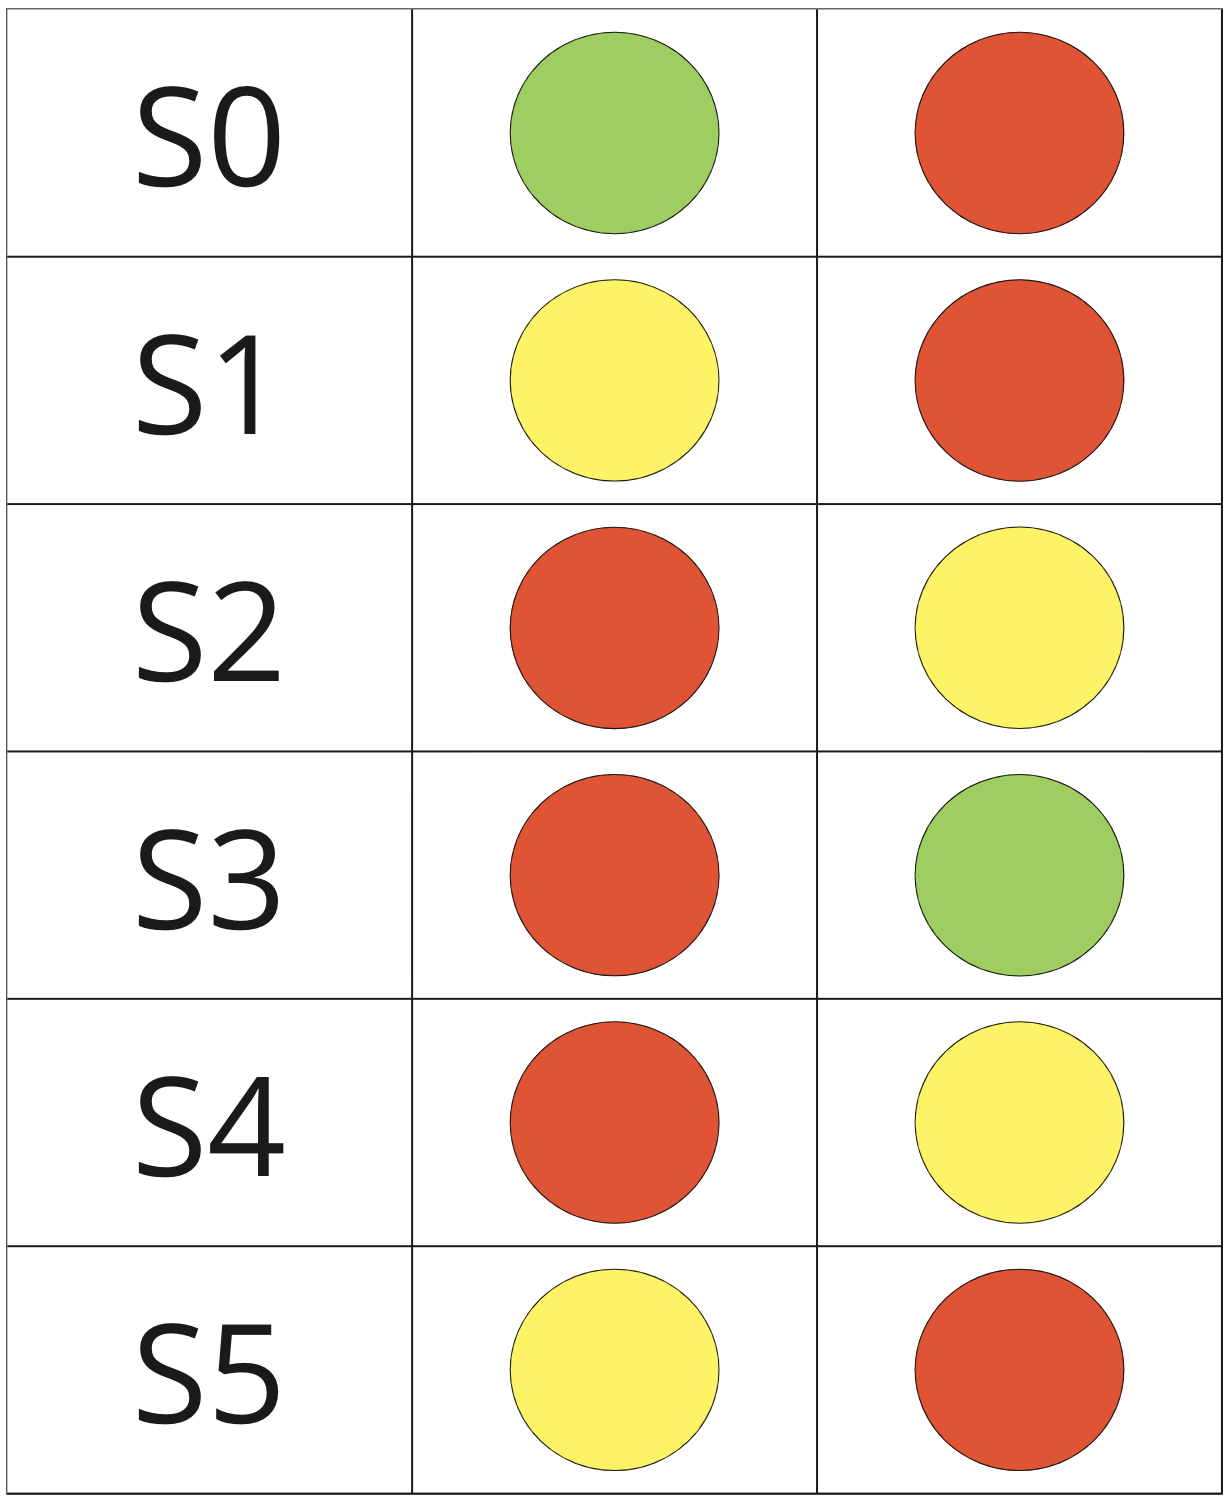
\includegraphics[width=0.4\textwidth]{figures/tabla_estados.png}
\caption{\label{fig:tabla_estados}Tabla de estados}
\end{figure}

El tiempo en amarillo será de 3 segundos mientras que en rojo y verde será de 30. A partir de esto, el sistema puede ser representado mediante el siguiente diagrama de estados

\begin{figure}[H]
\centering
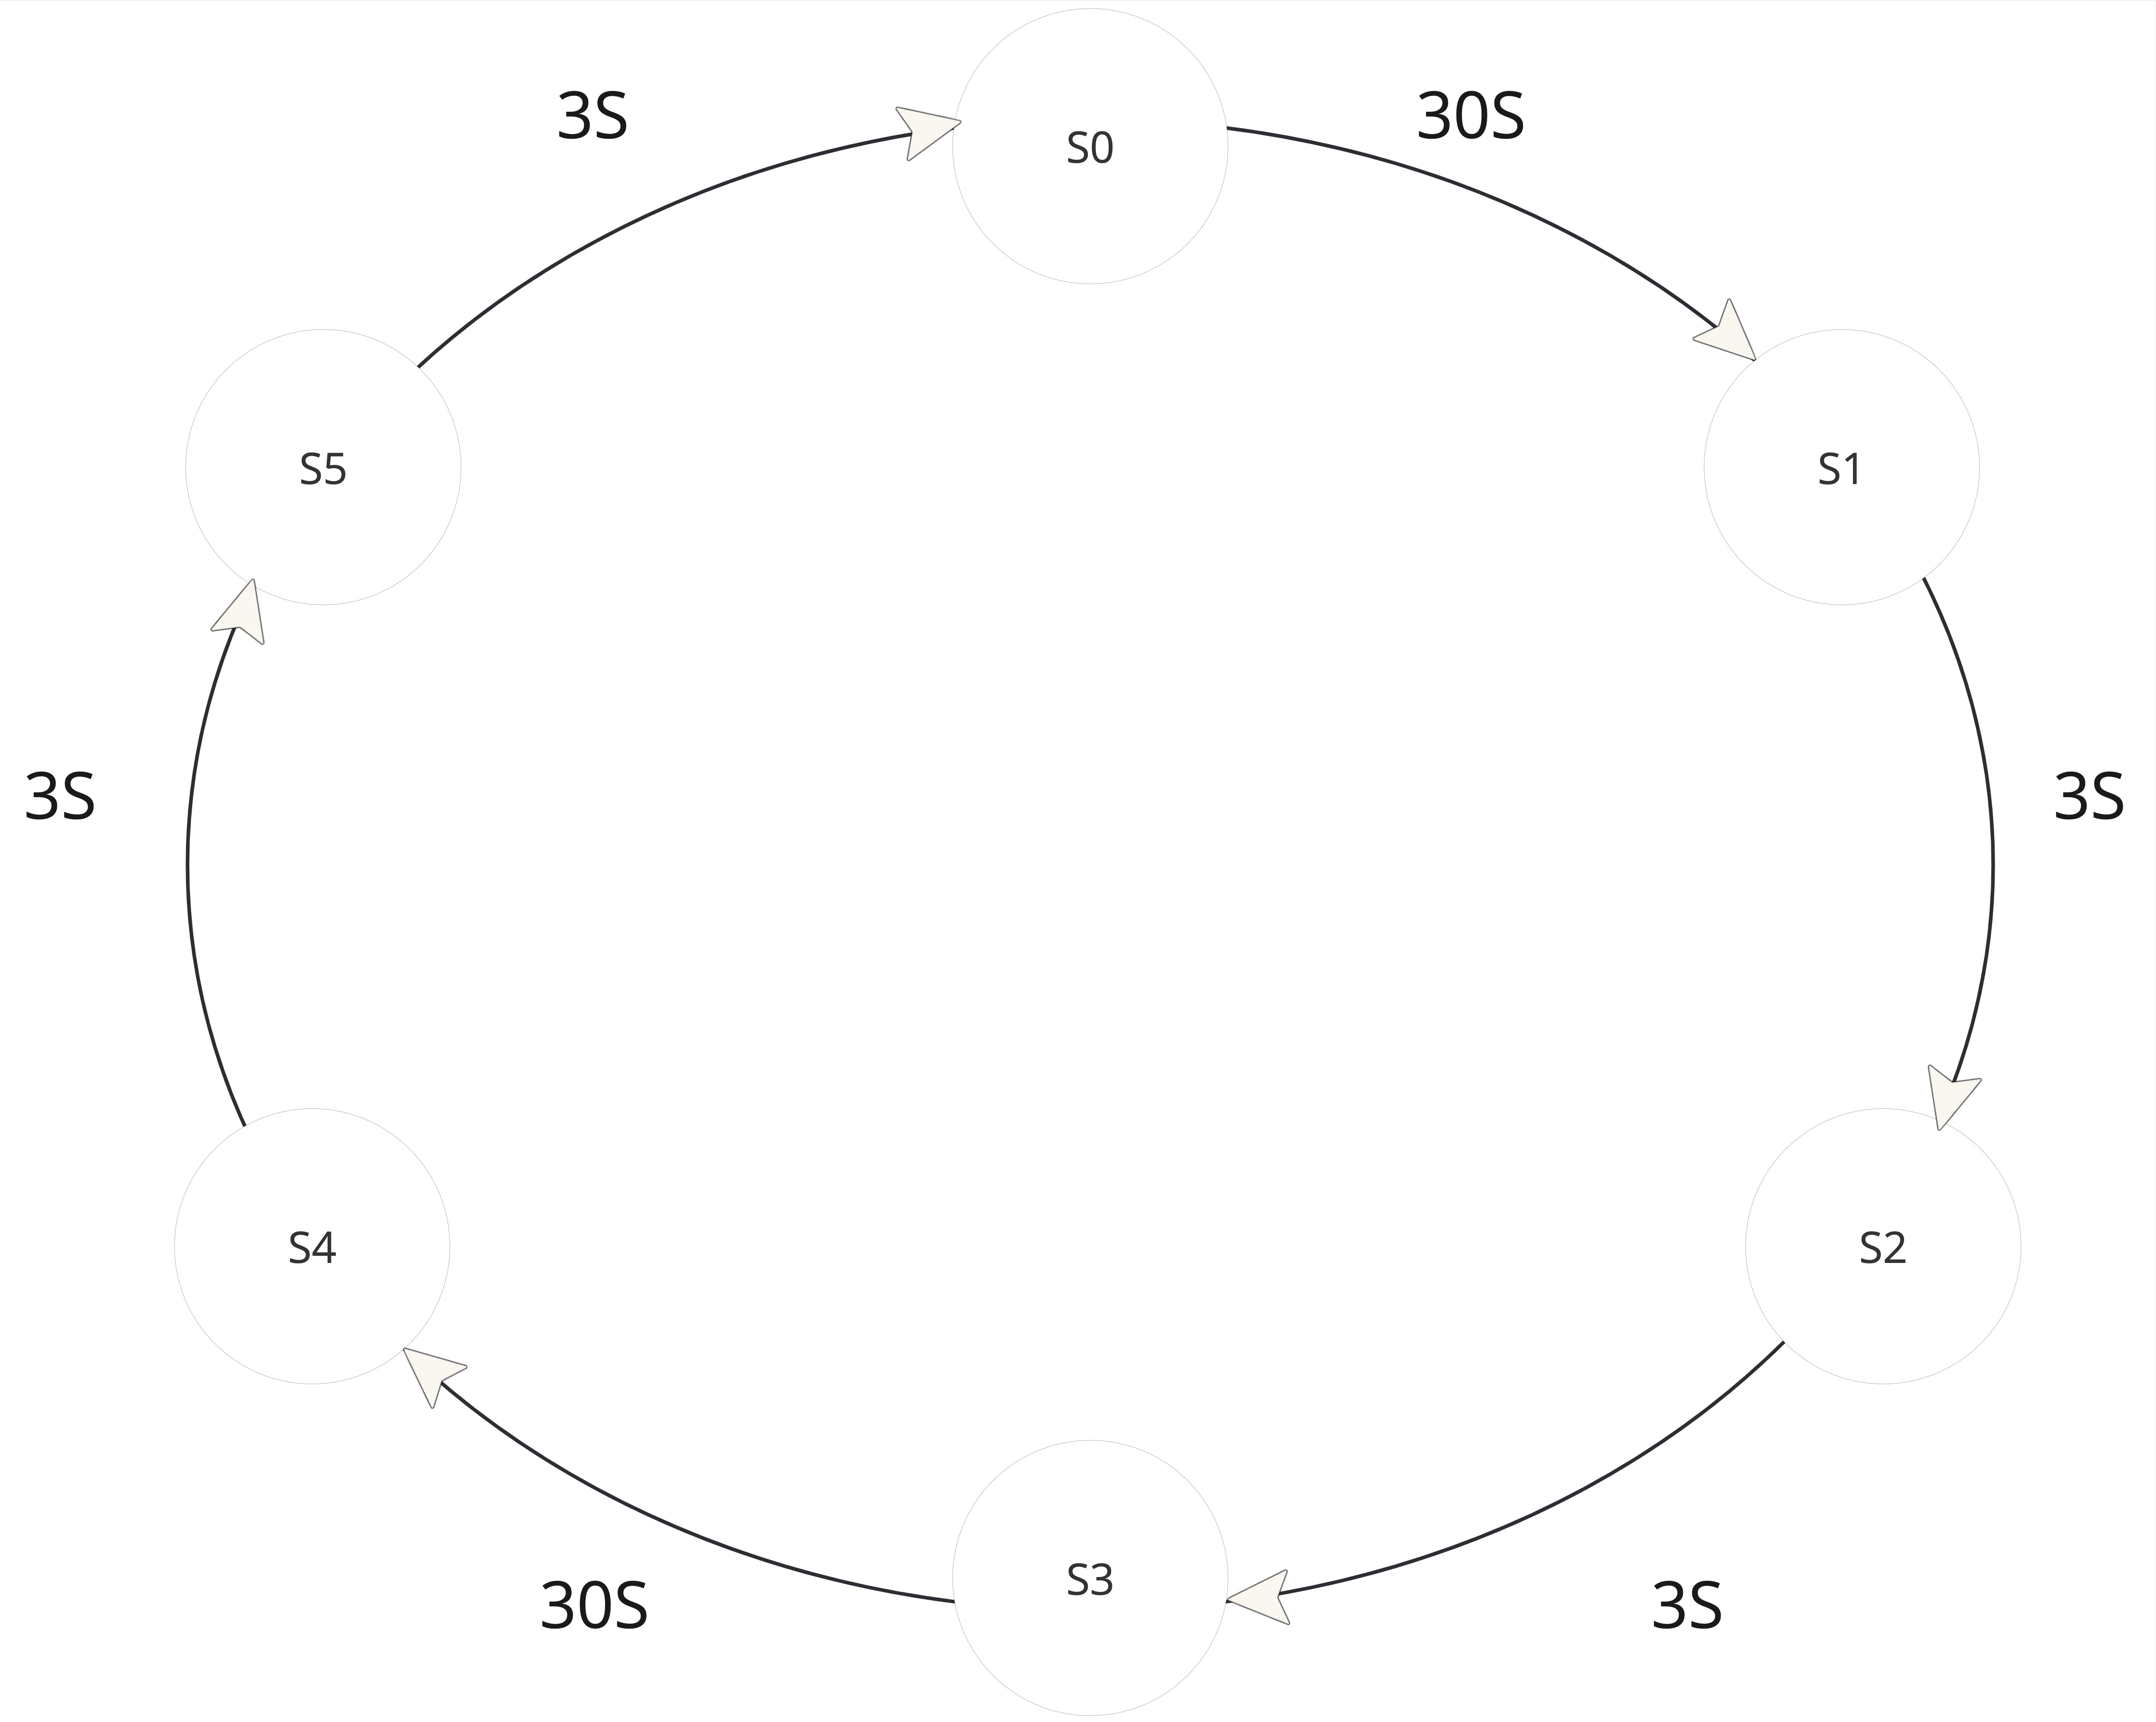
\includegraphics[width=0.6\textwidth]{figures/diagrama_estados.jpg}
\caption{\label{fig:diagrama_estados}Diagrama de estados}
\end{figure}

Para esto fueron desarrollados tres módulos principales

\subsection{Semáforos FSM}

Este módulo es responsable de controlar los estados del sistema de semáforos. Implementa una máquina de estados finitos (FSM) con seis estados diferentes, como se muestra en la Figura \ref{fig:tabla_estados}. Cada estado corresponde a una combinación específica de luces en los dos semáforos.

\subsection{Counter Dynamic}

Este módulo es un contador binario asincrónico que cuenta hasta un valor máximo. Cuando el contador alcanza su valor máximo, envía una señal indicando que sya se completo un ciclo de conteo.

\subsection{Counter Time}

También es un contador pero cuenta eventos basados en el tiempo. Usa el período del reloj y el período de tiempo especificado para determinar cuándo incrementar el contador. Calcula cuantos ciclos de reloj se deben contar a partir del tiempo dado, y usa el modulo \textit{counter dynamic} para contarlos. 

\subsection{Semaforos - Top Level}
En este modulo se instancia al \textit{semaforo\_fsm} además de dos contadores, uno para controlar el tiempo de duración del estado de 30 segundos y otro para controlar el tiempo de duración del estado de 3 segundos. El semáforo tiene dos señales de salida que son leídas por cada contador y les indica cuando debe empezar a contar. Además de dos señales de entrada enviadas por los contadores dando aviso de que el conteo finalizo y a partir de eso efectúa el cambio de estado. 

\section{Simulación}\label{sec:simulacion}
A continuación se puede ver una simulación del sistema, la misma se realizó usando la herramienta \textit{GHDL}. Para poder apreciar varios estados, se utilizó un valor de frecuencia de clock menor ($10 \, \text{Hz}$).

\begin{figure}[H]
\centering
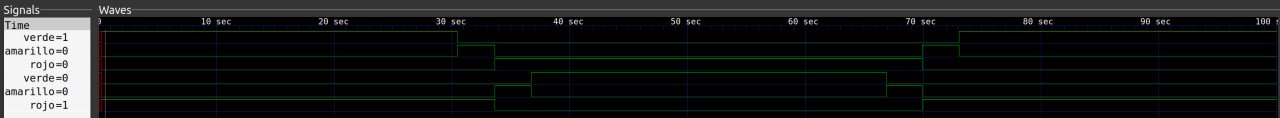
\includegraphics[width=0.8\textwidth]{figures/simulacion.jpeg}
\caption{\label{fig:simulacion}Simulación}
\end{figure}

\section{Síntesis}\label{sec:sintesis}
Se realizó la síntesis sobre el dispositivo \textit{FPGA xc7a15tftg256-1} con el software Vivado, se puede ver el esquemático a continuación con los módulos, entradas y salidas descriptos en la sección \ref{sec:desarrollo}.

\begin{figure}[H]
\centering
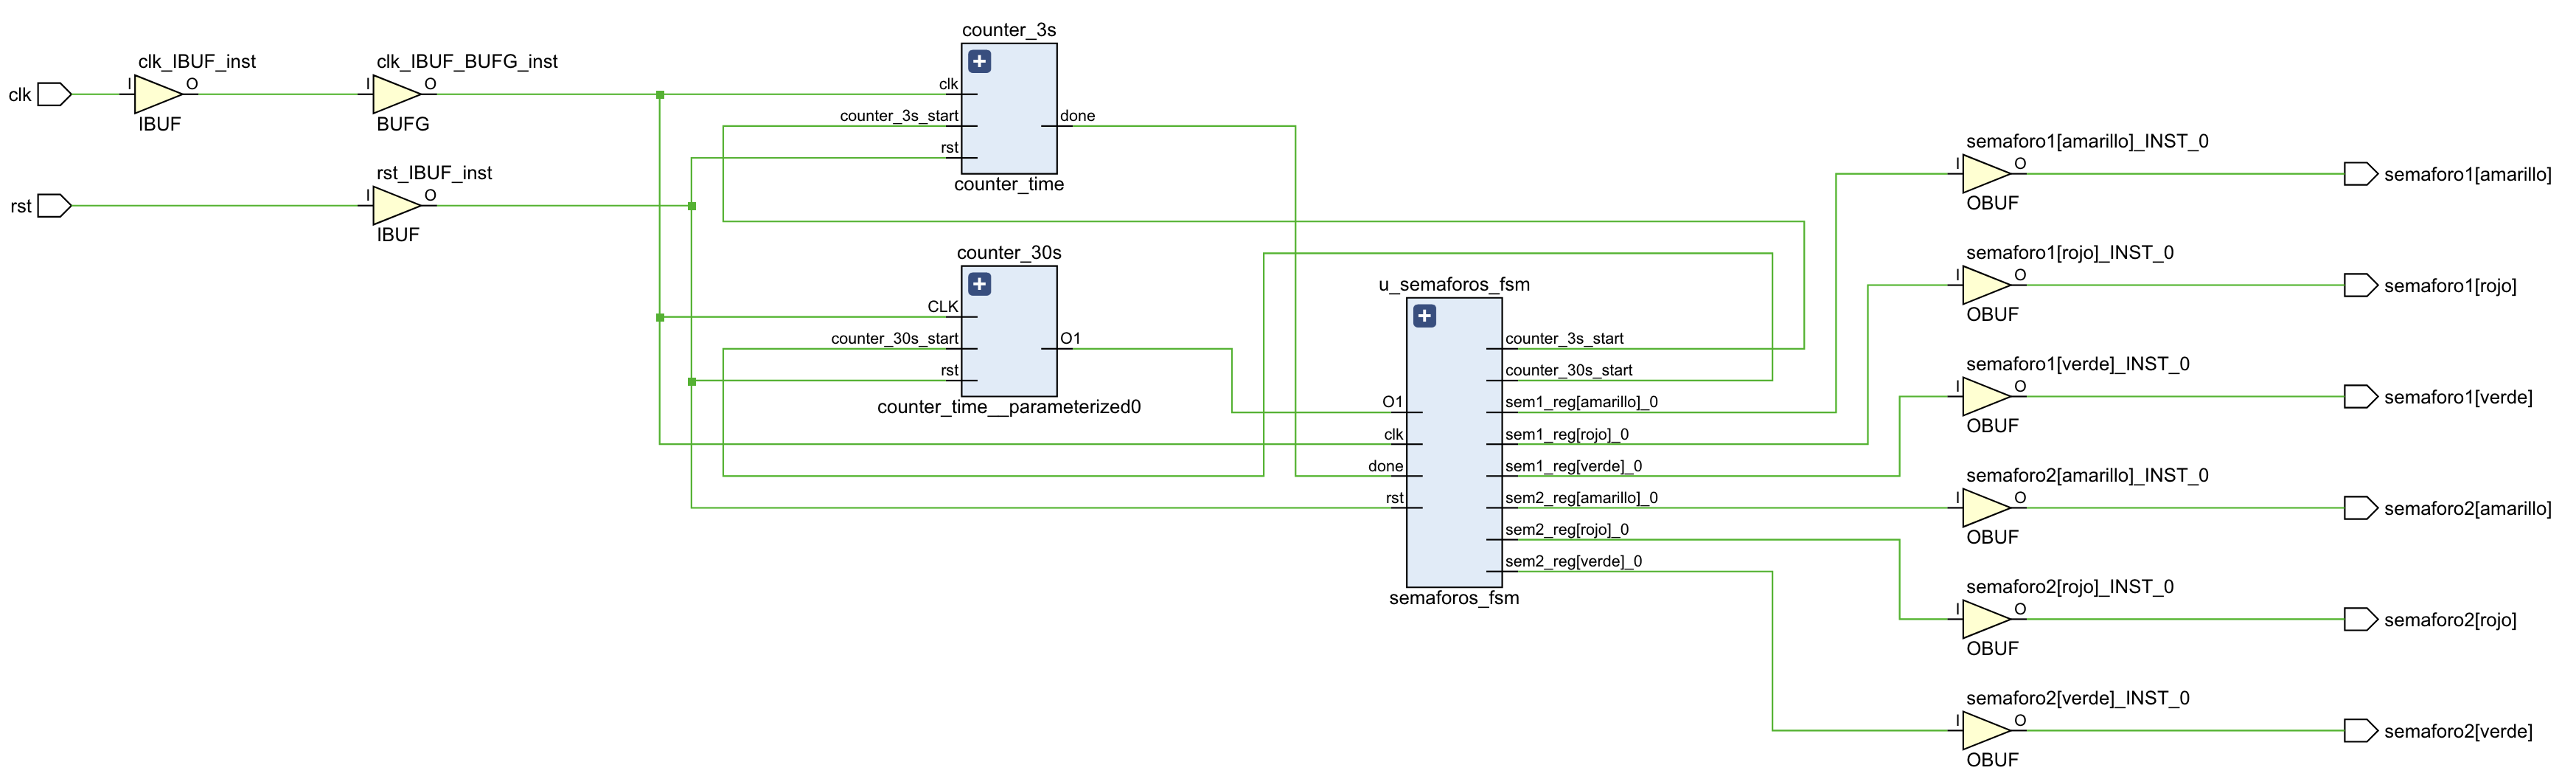
\includegraphics[width=1.1\textwidth]{figures/schematic.png}
\caption{\label{fig:simulacion}Síntesis}
\end{figure}


\newpage

\section{Anexo}\label{sec:anexo}
Se muestra a continuación el código desarrollado

\subsection{Código}

Top level:

\lstinputlisting{code/semaforos.vhd}
\lstinputlisting{code/tp1_pkg.vhd}
Semaforos\_FSM:

\lstinputlisting{code/semaforos_fsm.vhd}

Contadores:
\lstinputlisting{code/counter_dynamic.vhd}
\lstinputlisting{code/counter_time.vhd}

Test bench:
\lstinputlisting{code/tb.vhd}

\end{document}
